%------------------------------------------------------------------------------
% Template file for the submission of papers to IUCr journals in LaTeX2e
% using the iucr document class
% Copyright 1999-2013 International Union of Crystallography
% Version 1.6 (28 March 2013)
%------------------------------------------------------------------------------

\documentclass{iucr}              % DO NOT DELETE THIS LINE
\usepackage{color}
\usepackage{threeparttable}
\usepackage{amsmath}
\usepackage{todonotes}
\usepackage{booktabs}
\usepackage{xcolor}
\papertype{FA}

     %-------------------------------------------------------------------------
     % Information about journal to which submitted
     %-------------------------------------------------------------------------
     \journalcode{J}              % Indicate the journal to which submitted
                                  %   A - Acta Crystallographica Section A
                                  %   B - Acta Crystallographica Section B
                                  %   C - Acta Crystallographica Section C
                                  %   D - Acta Crystallographica Section D
                                  %   E - Acta Crystallographica Section E
                                  %   F - Acta Crystallographica Section F
                                  %   J - Journal of Applied Crystallography
                                  %   M - IUCrJ
                                  %   S - Journal of Synchrotron Radiation

\begin{document}                  % DO NOT DELETE THIS LINE

     %-------------------------------------------------------------------------
     % The introductory (header) part of the paper
     %-------------------------------------------------------------------------

     % The title of the paper. Use \shorttitle to indicate an abbreviated title
     % for use in running heads (you will need to uncomment it).

\title{Robust Characterization of sub-nanometer Cr/Sc Multilayers based on Complementary Measurements}
%\shorttitle{Short Title}

     % Authors' names and addresses. Use \cauthor for the main (contact) author.
     % Use \author for all other authors. Use \aff for authors' affiliations.
     % Use lower-case letters in square brackets to link authors to their
     % affiliations; if there is only one affiliation address, remove the [a].

\cauthor[a]{Anton}{Haase}{anton.haase@ptb.de}{}
\author[b]{Sa{\v{s}}a}{Bajt}
\author[a]{Philipp}{H{\"o}nicke}
\author[a]{Victor}{Soltwisch}
\author[a]{Frank}{Scholze}


\aff[a]{Physikalisch-Technische Bundesanstalt, Abbestr. 2-12, 10587 Berlin, \country{Germany}}
\aff[b]{Photon Science, DESY, Notkestr. 85, 22607 Hamburg, \country{Germany}}

     % Use \shortauthor to indicate an abbreviated author list for use in
     % running heads (you will need to uncomment it).

%\shortauthor{Soape, Author and Doe}

     % Use \vita if required to give biographical details (for authors of
     % invited review papers only). Uncomment it.

%\vita{Author's biography}

     % Keywords (required for Journal of Synchrotron Radiation only)
     % Use the \keyword macro for each word or phrase, e.g. 
     % \keyword{X-ray diffraction}\keyword{muscle}

%\keyword{keyword}

     % PDB and NDB reference codes for structures referenced in the article and
     % deposited with the Protein Data Bank and Nucleic Acids Database (Acta
     % Crystallographica Section D). Repeat for each separate structure e.g
     % \PDBref[dethiobiotin synthetase]{1byi} \NDBref[d(G$_4$CGC$_4$)]{ad0002}

%\PDBref[optional name]{refcode}
%\NDBref[optional name]{refcode}

\maketitle                        % DO NOT DELETE THIS LINE

\begin{synopsis}
Supply a synopsis of the paper for inclusion in the Table of Contents.
\end{synopsis}

\begin{abstract}
Cr/Sc multilayer systems can be used as near-normal incidence mirrors for the water window spectral range. We show that a detailed characterization of these multilayer systems  with 400 bilayers of Cr and Sc each with individual layer thicknesses below $<1$ nm is attainable by the combination of several analytic experiments. We used EUV- and X-ray reflectivity measurements, resonant EUV reflectivity across the Sc L-edge as well as X-ray standing wave fluorescence measurements. The parameters of our multilayer model were determined based on a particle swarm optimizer and validated using a Markov-chain Monte Carlo maximum likelihood approach. For the determination of the interface roughness power spectral density diffuse scattering measurements were conducted.
\end{abstract}


     %-------------------------------------------------------------------------
     % The main body of the paper
     %-------------------------------------------------------------------------
     % Now enter the text of the document in multiple \section's, \subsection's
     % and \subsubsection's as required.

\section{Introduction}

The wavelength range of the so called ``water window'' between $2.2$ nm and $4.4$ nm wavelength is of special interest for many scientific applications. Radiation in this spectral range shows low absorption in water, while it is absorbed by many elements naturally occurring in organic molecules such as proteins \cite{WaterWindowBioRelevance}. This allows to study those biological systems in water, where many proteins are biologically active. High-reflective optics are required to take advantage of the high resolution possible due to the short wavelength in direct imaging of these samples \cite{waterwindow_mirrors_1,Legall:12}.

The strong absorption of soft X-ray radiation in most materials poses a challenge in the fabrication of such optics. Refractive optics are almost impossible due to the high absorption in solids. The same holds for reflective optics close to normal incidence, where reflectivities of well below $10^{-4}$ can be expected from a single surface of all materials \cite{henke}. A candidate system for building high-reflective mirrors for short wavelength is a layered structure with alternating materials of significantly different refractive index \cite{SpillerMultilayer}. Those multiple repeated bilayer systems constitute an artificial one-dimensional Bragg crystal. Their layer layout, more specifically the total layer thickness $D$ of a single layer period, is intrinsically related to the desired peak reflectivity wavelength and incidence angle. Those systems are well established as mirrors for EUV wavelength of $13.5$ nm, where they reflect more than $70\%$ of the radiation at angles of incidence of $6^\circ$ from the surface normal with a choice of Mo and Si as layer materials. Theoretical calculations show that constructing multilayer mirrors in the water window spectral range for angles of incidence of $1.5^\circ$ allows peak reflectivities above $50\%$ \cite{Schafers:98}. A typical choice of materials for these bilayer systems are Cr and Sc for wavelength above $3.1$ nm \cite{Salashchenko19977, Schafers:98}. The proximity to the Sc L-edge causes the required significant difference in the refractive index due to anomalous dispersion while maintaining relatively low absorption. In order to function as a one-dimensional Bragg crystal those layer systems demand a high quality of the layer interfaces. Chemically abrupt and smooth interfaces are required to reach high reflectivities and to minimize loss processes such as diffuse scattering or contrast decrease due to interdiffusion. This requirement becomes even more stringent when moving towards shorter wavelength due to the necessary reduction in layer thickness for fulfilling the Bragg condition.
The relative influence of interface morphology and interdiffusion as loss mechanisms for peak reflectivity rise in importance compared to established Mo/Si multilayer systems with significantly larger layer thicknesses. The measured peak reflectivity of state-of-the-art Cr/Sc multilayer systems designed for the above specifications score at reflectivities below $20\%$, less than half of the theoretically possible value (cf.~inset~Fig.~\ref{fig:EUV_XRR_reflectivity}) \cite{Eriksson:03, doi:10.1117/12.505688}.

Roughness causes diffuse scattering out of the specular beam direction \cite{sinha_scattering_natural_tool}. Interdiffusion on the other hand reduces the optical contrast, i.e.~the local difference in the refractive index thereby reducing the reflectivity at each interface \cite{nakajima_interdiffusion}. In order to gain a deeper understanding of the interface morphology a characterization of these samples is required. The inspection of diffusely scattered light is a natural tool for the investigation of the roughness at the interfaces. An at-wavelength measurement of in-plane diffuse scattering contributions contains information on the interface morphology. An important advantage of this analysis as compared to established methods for interface characterization of thin films such as GISAXS \cite{Levine:pn0068} is that the angle of incidence is close to the surface normal. This enables the possibility to locally investigate the multilayer stack even for strongly curved surfaces, e.g.~in case of focusing optics.


Standard characterization methods such as EUV reflectivity and X-ray reflectivity with simple binary layer models have proven useful for the characterization of similar multilayer systems, e.g.~Mo/Si mirrors designed for $13.5$ nm wavelength \cite{Lim2001, bajt_mosi_crstallization, braun_mosi_different_barrier_layers}. However, these systems typically have thicknesses of $3$ -- $4$ nm within a single period for the Mo and Si layers. With the efforts of reducing the desired peak reflectivity wavelength, those methods fail in yielding information to build simple models that describe measured reflectivities \cite{Yakunin:14}. The results of the analysis based on the standard binary model of a Cr/Sc multilayer with a Sc to Cr ratio of $\Gamma_\text{Sc}=0.48$ are shown in Fig.~\ref{fig:EUV_XRR_reflectivity}. The individual layer thicknesses for this sample were fitted to be $d_\text{Cr} = 0.81$ nm and $d_\text{Sc}= 0.75$ nm. While the EUV reflectivity curve (cf.~inset in Fig.~\ref{fig:EUV_XRR_reflectivity}) shows a good agreement with the measured data, there is a significant offset in case of the XRR measurement with the (binary) model derived from the EUV reflectivity experiment. Even a simultaneous analysis could not yield a consistent result. In a strictly binary model with a layer thickness ratio of $\Gamma_\text{Sc}\approx 0.5$, the second Bragg peak is suppressed due to symmetry reasons. This, however, is a clear mismatch with the experimental observation as seen in the comparison of the fitted and measured XRR curves in Fig.~\ref{fig:EUV_XRR_reflectivity}.
\begin{figure}
  \centering
  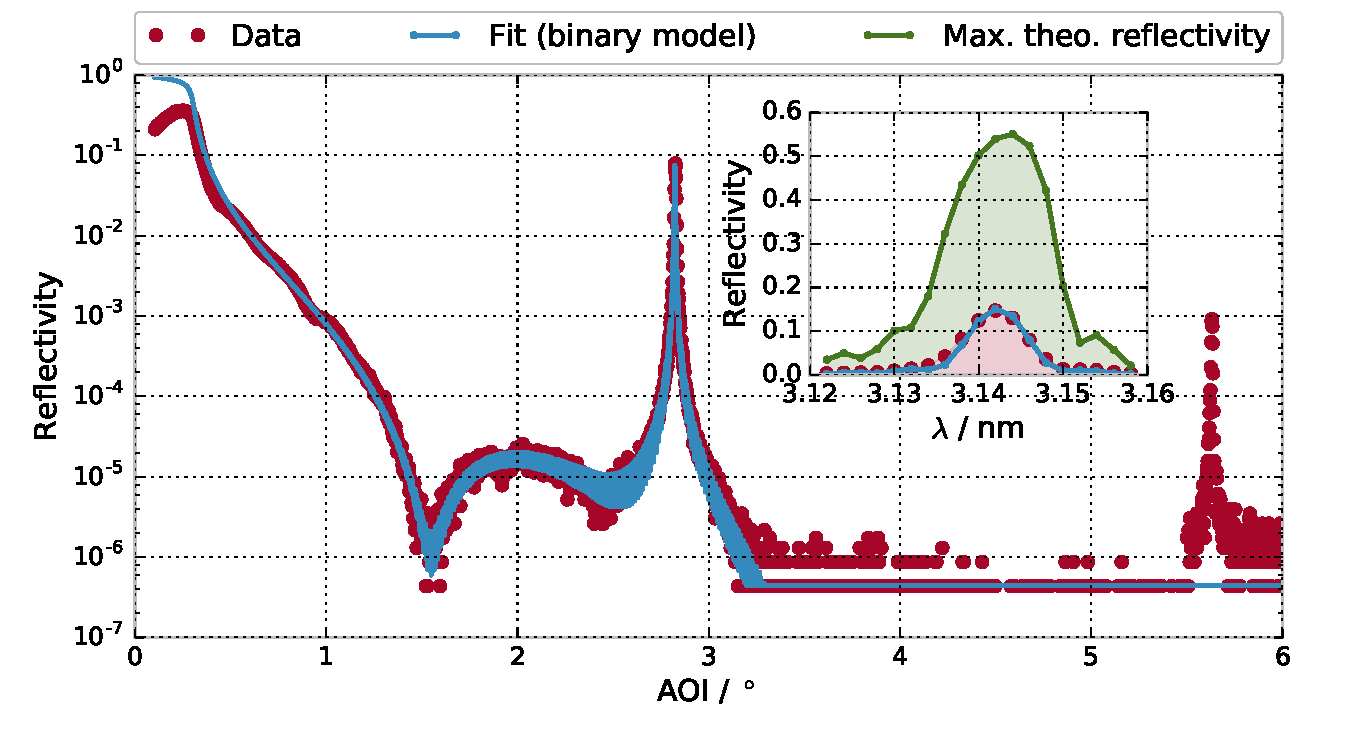
\includegraphics[width=\textwidth]{images/binary_model_and_theo_refl}
  \caption{Theoretical and experimental X-ray reflectivity curves based on the simple binary model. The optimal model based on the analysis of the EUV reflectivity (cf.~inset) shows a clear mismatch with the measured XRR curve in the second Bragg peak. Inset: Fitted experimental EUV reflectivity curves across the wavelength of the radiation impinging at $1.5^\circ$ from normal based on a simple binary model. The green curve shows the maximum possible reflectivity assuming a perfect layer system.
}
  \label{fig:EUV_XRR_reflectivity}
\end{figure}

The reason for this mismatch is the growing relative influence of disturbances at the interfaces potential breaking the symmetry condition. This needs to be taken into account explicitly in the model and leaves the simple binary approach as an insufficient description of the physical situation. The increase of parameters required to describe a more realistic model also pose a requirement on information gained through analytic experiments. We thus apply a set of different experimental methods to obtain a consistent reconstruction of the multilayer structure with a non-destructive approach. We demonstrate that in case of layer systems in the sub-nanometer regime, a combined analysis of this experiments is required. For this, we derive a sophisticated model considering graded interface profiles and intermixing of the two materials. The validation of the derived model is conducted by applying a Markov-chain Monte Carlo sampler.



\section{Experimental details} \label{sec:experimental}

The multilayer samples were prepared at the DESY X-ray multilayer laboratory by DC magnetron sputtering \cite{crsc_thermal_bajt} \todo{more info}. They are composed out of alternating layers of Cr and Sc with periodic replication of the bilayer stack by $N=400$ times. The substrates are superpolished Si wafer pieces. The sample dimensions measure approximately $(20 \times 20)$ mm$^2$. The multilayer mirrors were designed to reflect radiation in the water window energetically below the Sc L-edge close to $3.1$ nm wavelength at an angle of incidence of $1.5^\circ$ from the surface normal.

The characterization via XRR was conducted in the DESY laboratory using a high-resolution X-ray diffractometer. It is equipped with a high-resolution goniometer and uses the Cu-K$_\alpha$ wavelength. The reflectivity experiments were recorded using a counting detector in grazing incidence geometry measured at angles of incidence from $\alpha_i=0^\circ$ to $\alpha_i=3^\circ$. The dynamic range achieved in the measurement ranged down to a reflectivity of $10^{-6}$. Due to the low layer thickness in each period of the multilayer sample, only two Bragg peaks at most could be measured with this technique. All higher order peaks were below the detection threshold of $10^{-6}$ in reflected intensity.

All other experiments were conducted in the laboratory of the Physikalisch-Technische Bundesanstalt (PTB) at the electron storage ring BESSY II in Berlin-Adlershof. The EUV reflectivity (cf.~inset Fig.~\ref{fig:EUV_XRR_reflectivity}) and resonant EUV reflectivity measurements (REUV, cf.~Fig.~\ref{fig:REUV_XRF_data}(a)) were done in the new ellipso-scatterometer at the soft X-ray beamline \cite{Beckhoff2009} under ultra high vacuum (UHV) conditions. The accessible spectral range at the SX700 plane grating monochromator ranges from $0.8$ nm to $25$ nm. The samples were mounted on a 6-axis goniometer sample holder. The movable detector arm in combination with the goniometer allows measurements in in-plane and out-of-plane geometry. For the resonant EUV (REUV) reflectivity measurements across the Sc L-edge the wavelength was kept fixed while performing a specular angular reflectivity scan ($\Theta$/$2\Theta$-scan). The X-ray standing wave experiments or X-ray flourescence experiments (XSW/XRF), respectively, were done at the four-crystal monochromator beamline (FCM), where energies up to $10$ keV well above the K-absorption edges of Sc and Cr are accessible. The end station is a dedicated X-ray flourescence measurement chamber also under UHV. The fluorescence data was taken at a selected photon energy of $E=6.25$ keV, above the Cr edge. The relative fluorescence yield from the Sc and Cr K-edges, respectively, is shown in Fig.~\ref{fig:REUV_XRF_data}(b) and~\ref{fig:REUV_XRF_data}(c). The grazing angle of incidence was varied across the resonance condition for the first Bragg peak to excite the standing wave field inside the multilayer.
\onecolumn
\begin{figure}
  \centering
  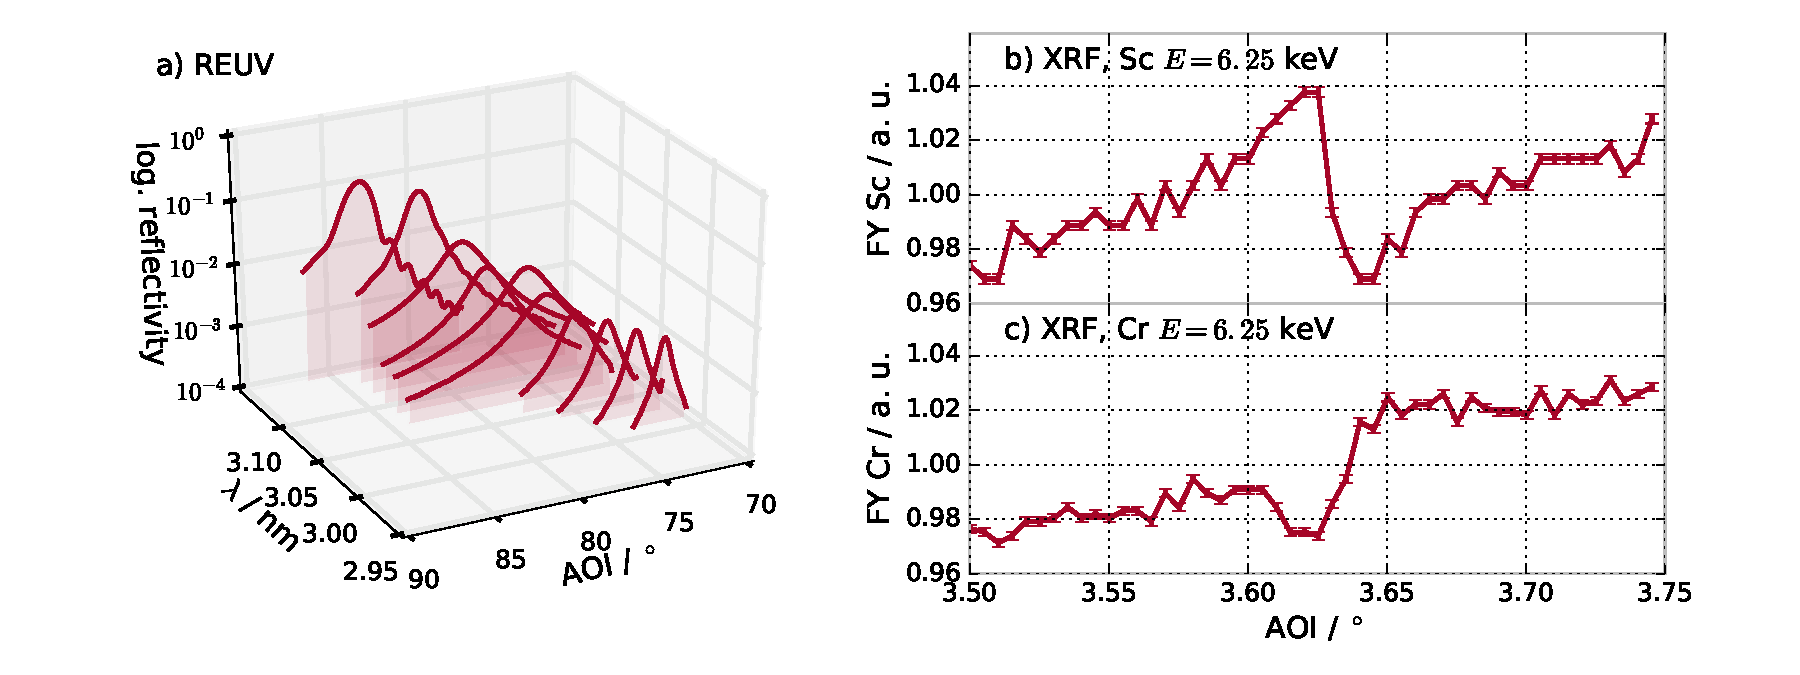
\includegraphics[width=\textwidth]{images/reuv_xrf_data}
  \caption{a) Resonant EUV reflectivity across the Sc L-edge. Several angular reflectivity scans have been performed at selected wavelength across the Sc L-edge. b) and c) X-ray standing wave fluorescence recorded across the first Bragg peak by varying the angle of incidence for the Sc signal (b) and the Cr signal (c). Both curves were recorded simultaneously at an excitation energy of $E=6.25$ keV. The data is shown in relative (arbitrary) units of intensity.}
  \label{fig:REUV_XRF_data}
\end{figure}
\twocolumn

The diffuse scattering measurements were performed with a detector angle of $2\Theta = 3^\circ$ with respect to the incoming beam, while rocking the sample from $\Theta = 1.5^\circ - 7.0^\circ$ and tuning the wavelength from $\lambda = 3.0 - 3.4$ nm at each angular position. Diffuse scattering measurements close to near-normal incidence allow for local measurements due to the small beam spotsize on the sample. This measurement technique allows to obtain a reciprocal space map of the diffuse scattering distribution as shown in Fig.~\ref{fig:diffuse_meas} below.


\section{Theoretical background} \label{sec:matrix_formalism}

\subsection{Matrix formalism: EUV, REUV, XRR} \label{subsec:matrix_formalism}

The EUV and X-ray reflectivity is calculated based on the well established matrix formalism \cite{PrinciplesOfOptics}. The reflection $r_{id}^{(j)}$  and transmission $t_{id}^{(j)}$ at each interface $j$ is given by the Fresnel coefficients
\begin{align}
	r_{id}^{(j)} &= \frac{k_z^{(j)} - k_z^{(j+1)}}{k_z^{(j)} + k_z^{(j+1)}}\text{,} \\
	t_{id}^{(j)} &= \frac{2 k_z^{(j)}}{k_z^{(j)} + k_z^{(j+1)}}\text{,} 
\end{align}
where $k_z^{(j)}$ is the complex $z$-component of the incident wave vector $\vec{k}$ at the $j$th interface. Its value is calculated according to Snell's law at each interface taking into account the complex indices of refraction $n^{(j)}$.
In order to account for roughness induced loss of specular reflectivity, modified Fresnel coefficients based on a Nevot-Croce factor $\sigma_r$ are considered at each interface \cite{nevot_croece}. We approximate the interface mean square roughness to be identical at each interface, i.e.~$\sigma_j \equiv \sigma_r\text{,} \, \forall j$. Considering different roughness at each interface would increase the number of variable parameters in the model by the amount of interfaces and thus lead to overdetermination. The analysis of the diffuse scattering from Mo/Si multilayer systems has shown a high correlation of the interface roughness throughout the stack \cite{Haase:14}, which supports the approximation of identical roughness made here. With this approximation the modified Fresnel coefficients assuming a error function type interface profile are given by
\begin{align}
	r^{(j)} &= r_{id}^{(j)} \exp(-2 k_z^{(j)} k_z^{(j+1)} \sigma_r^2)\text{,} \nonumber \\
	t^{(j)} &= t_{id}^{(j)} \exp((k_z^{(j)} - k_z^{(j+1)})^2 \sigma_r^2/2) \text{.} \label{eqn:modified_fresnel}
\end{align}

The electric fields at each interface are then related with the fields at the next interface through the field propagation matrix $M_j$ \cite{mikulik1997x}
\begin{align}
M_j = \frac{1}{t^{(j)}}
\begin{pmatrix}
1 & r^{(j)} \\
r^{(j)} & 1
\end{pmatrix}
\begin{pmatrix}
e^{-i k_z^{(j+1)} d_j} & 1 \\
1 & e^{i k_z^{(j+1)} d_j}
\end{pmatrix}
\text{,} \label{eqn:field_propagation_matrix}
\end{align}
The fields inside the multilayer stack, as well as inside the substrate and the vacuum are given by Eq.~\eqref{eqn:field_propagation_equation}.
\begin{align}
\begin{pmatrix}
E_0 \\
E_R
\end{pmatrix} &=
\prod\limits_{j} M_j
\begin{pmatrix}
E_T \\
0
\end{pmatrix} \text{.} \label{eqn:field_propagation_equation}
\end{align} 
The total wave field is represented by a two dimensional vector. The upper component describes the amplitude of the wave propagating towards the substrate and the lower component describes the reflected wave amplitude propagating towards the vacuum. Iterative application of the field propagation matrix yields the electric field amplitudes $E$ at each interface for both propagation directions. The solution is obtained by starting from the condition of a known incoming wave amplitude $E_0$ and the lack of a reflected wave amplitude inside the substrate.

The components $E_T$ and $E_R$ describe the transmitted and reflected field amplitudes inside the vacuum and the substrate, respectively.
Normalized reflectivity $R$ and transmitivity $T$ values for the EUV, REUV and XRR measurements are obtained from the field calculation by dividing the calculated values with the initial field amplitude $E_0$
\begin{align}
R &= |E_R/E_0|^2\text{,} \nonumber\\
T &= |E_T/E_0|^2 \text{.} \label{eqn:refl_trans}
\end{align}

\subsection{X-ray standing wave fluorescence analysis} \label{subsec:xrf_formalism}

The calculation of the relative fluorescence signal XRF for either element in the multilayer stack is done by discrete numerical integration of the product of the total electric field intensities $I \propto |E(z)|^2 = | E_r(z) + E_t(z)|^2$ with the relative density profile of the elements $\rho(z) = \rho_\text{Sc}(z)$ or $\rho(z) = \rho_\text{Cr}(z)$, respectively, along the surface normal of the sample, i.e.~
\begin{align}
 I_\text{XRF}\propto \int\limits_0^{D_\text{total}} |E(z)|^2 \rho(z) \,\text{d}z \text{,}
\end{align}
where the total thickness $D_\text{total}$ of the multilayer stack is given by $D_\text{total} = N D+D_\text{cap}$ with $N$ being the number of multilayer periods, $D$ the thickness of a single period and $D_\text{cap}$ the total tickness of all capping layers and $z$ is the coordinate along the surface normal with respect to the substrate surface. The total electric field $E(z)$ is evaluated at discrete points $z_j$ inside the multilayer including the interfaces according to Eq.~\eqref{eqn:field_propagation_equation}, while the distance between two sample points is significantly less than the thickness of a single layer to approximate the continous wave intensity dependence along $z$.
\subsection{Distorted-wave Born approximation} \label{subsec:dwba_formalism}

The theoretical analysis of the diffuse EUV scattering data obtained has been done based on the distorted-wave Born approximation (DWBA) \cite{PhysRevB.49.10668,PhysRevB.47.15896}. Here, the interface roughness is considered to be a small distortion on the solution of the perfect multilayer system. We apply that to diffuse scattering measurements near-normal incidence, where dynamic effects become important and need to be considered in order to obtain the power spectral density (PSD) of the interface morphology. Our approach is described in detail in \cite{Haase:14}. Following from Eq.~\eqref{eqn:field_propagation_equation} and Eq.~\eqref{eqn:refl_trans} The explicit transmitted and reflected fields at the interfaces are given by
\begin{align}
	E_t^{(j)}(z) &= T_{j} e^{i k_z^{(j)} z} \text{,} \\
	E_r^{(j)}(z) &= R_{j} e^{-i k_z^{(j)} z} \text{,}
\end{align}
where $T_{j}$ and $R_{j}$ are the transmitted and reflected field amplitudes at each interface, respectively. The fields are calculated based on the matrix formalism described above using the undisturbed system, i.e.~the ideal Fresnel coefficients instead of the modified coefficients already including a correction for roughness. The solution serves as the undisturbed wave field entering the DWBA calculation. The diffuse scattering intensity is then given by
\onecolumn
    \begin{align}
        \Big(\frac{d \sigma}{d \Omega}\Big) = &\Bigg[\frac{A \pi^2}{\lambda^4}\sum \limits_{j=1}^{N}\sum \limits_{i=1}^{N} (n_j^2 - n_{j+1}^2)^* (n_i^2 - n_{i+1}^2)\Big( (T^{(1)}_j + R^{(1)}_j)^* (T^{(2)}_j + R^{(2)}_j)^* \nonumber \\ &\qquad\times(T^{(1)}_i + R^{(1)}_i) (T^{(2)}_i + R^{(2)}_i) \Big) \exp\Big(-i q_x \tan \beta (z_i-z_j)\Big) c^\perp_{i j}\Bigg]\,\, C(q_x) \text{,} \label{eqn:dwba}
    \end{align}
\twocolumn
taking into account all first-order dynamic effects. Here, $n_j$ represents the complex refractive index inside each layer, $A$ respresents the illuminated area, $\lambda$ respresents the wavelength of the impinging radiation, $\beta$ indicates the angle at which correlated roughness replicates from interface to interface throughout the stack and $z_i$ the position of the interface, both with respect to the surface normal. The leading term of Eq.~\eqref{eqn:dwba} contained within rectangular brackets can be considered as a multilayer enhancement factor separating the contributions of the multilayer nature and the vertical correlations of the sample from the roughness at the interfaces isolated in the PSD $C(q_x)$. The scattering distribution is calculated in reciprocal space coordinates or the wave vector transfer $q$ given by
\begin{align}
	q_x &= \frac{2 \pi}{\lambda} \big(\sin(\alpha_f) - \sin(\alpha_i)\big) \text{,}\\
	q_z &= \frac{2\pi}{\lambda} \big(\cos(\alpha_f) + \cos(\alpha_i)\big) \text{,} 
\end{align}
where $\alpha_i$ is the angle of incidence from normal and $\alpha_f$ is the scattering angle.
The roughness properties of the interfaces is contained in the replication factor $c_{ij}^\perp$ \cite{spiller1993multilayer} and the effective one-dimensional power spectral density $C(q_x)$. There exist several PSD models in literature, e.g.~by Sinha et al.~\cite{PhysRevB.38.2297}, for single rough interfaces or surfaces, respectively. Due to the low thickness of the individual layers we make the approximation of identical statistical properties of each interface with respect to the roughness, i.e.~we assume identical PSDs. We follow the definition of de Boehr et al.~\cite{deBoerLateralCorrelation,PhysRevB.51.5297} which yields a closed analytic form of the PSD for a fractal roughness model
\begin{align}
    C(q_x) = \frac{4 \pi H \sigma_r^2 \xi_\parallel^2}{(1+|q_x|^2\xi_\parallel^2)^{1+H}} \text{,} \label{eqn:psd} 
\end{align}
where $\sigma_r$ is the root mean square roughness, $H$ is the Hurst factor describing the jaggedness of the interface and $\xi_\parallel$ is the in-plane correlation length. The replication factor $c_{ij}^\perp$ is given by
\begin{align}
c_{ij}^\perp(q_x) =  \exp\Bigg(-\sum \limits_{n = \text{min}(i,j)}^{\text{max}(i,j)-1}d_n/\xi_\perp(q_x) \Bigg)\text{,}
\end{align}
where $d_n$ is the thickness of the $n$th layer and $\xi_\perp(q_x) = \xi_\perp/q_x^2$ is a spacial frequency dependent vertical correlation length at which the replication factor has decreased to $1/e$.


\section{Improved model for robust reconstruction} \label{sec:model}

Instead of the simple binary layer model a gradual interface model is introduced to better reflect the realistic electron density profile due to interdiffusion and roughness. A corresponding profile is shown in Fig.~\ref{fig:CrScModel} for illustration in comparison to the binary model.
\begin{figure}
  \centering
  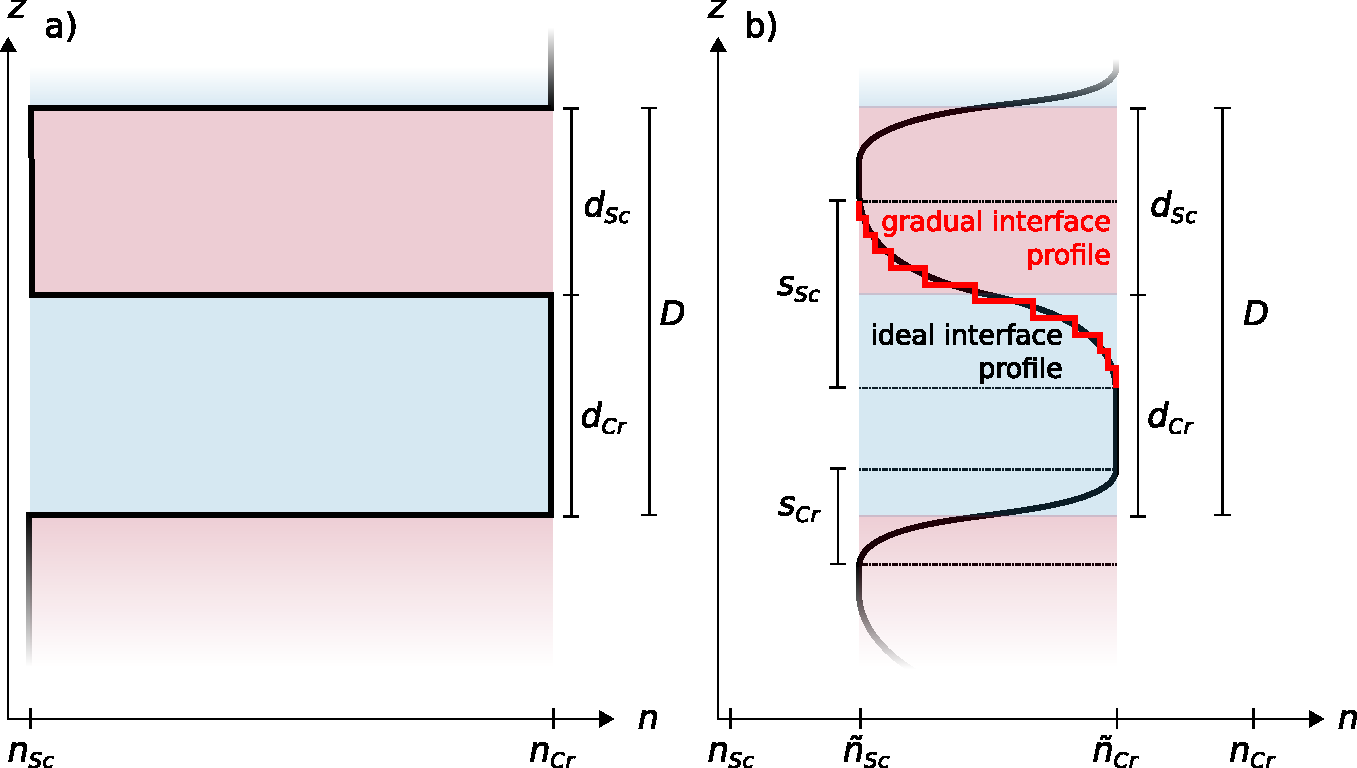
\includegraphics[width=\textwidth]{images/CrSc_model}
  \caption{a) Binary Cr/Sc multilayer model with total period thickness $D$ and the individual layer thicknesses $d_\text{Sc}$ and $d_\text{Cr}$. b) Gradual interface model with explicit gradual interfaces following a sinusoidal profile. The ideal interface profile is approximated through discrete sublayers as indicated in red forming the actual gradual interface profile entering the electric field calculations. The thickness of the interdiffusion zones can differ for the top and bottom interface in each period. Their total thicknesses is given by $s_\text{Sc}$ and $s_\text{Cr}$. Due to intermixing across multiple periods a reduction of the index of refraction for each material towards the average of both materials is possible. The effective index of refraction for both materials is thus given by $\tilde{n}_\text{Sc}$ and $\tilde{n}_\text{Cr}$, respectively.}
  \label{fig:CrScModel}
\end{figure}
The calculation of the electromagnetic fields is then conducted based on this model with the matrix formalism introduced in the preceding section. The interface region with sinusoidal profiles is sampled with a fixed number of equally spaced points in $z$-direction effectively creating a region of thin sublayers with gradually changing index of refraction. The parameters of our multilayer model are listed in Table~\ref{tbl:parametrization},
\begin{table}
\centering
\caption{Multilayer parametrization and parameter limits}
\label{tbl:parametrization}
\begin{tabular}{@{}llll@{}}
\toprule
Parameter & Definition & Lower bound & Upper bound\\ \midrule
$D$ / nm & $= d_\text{Sc} + d_\text{Cr}$ & 1.5&1.6 \\ 
$\Gamma_{Sc}$ & $= d_\text{Sc} / D$&0.0 &1.0 \\ 
$\sigma_d$ / nm&$=s_\text{Sc} + s_\text{Cr}$&0.0 & 1.6\protect\footnotemark\\ 
$\Gamma_\sigma$ &$= s_\text{Sc} / \big(s_\text{Sc} + s_\text{Cr}\big)$& 0.0& 1.0\\ 
$\eta$ &layer intermixing& 0.0& 1.0\\ 
$\sigma_r$ / nm & r.m.s.~roughness& 0.0& 0.5\\ 
$\rho_{Sc}$ &Sc density w.r.t.~bulk density & 0.5& 1.0\\ 
$\rho_{Cr}$ &Cr density w.r.t.~bulk density& 0.5& 1.0\\ 
 \bottomrule
\end{tabular}
\end{table}
\footnotetext{The maximum value of the interdiffusion layer thickness is limited due to the thicknesses of the individual layers $d_\text{Sc}$ and $d_\text{Cr}$ through the relation $\sigma_d \leq D$}
%\begin{align}
%	\text{Multilayer parametrization}
%    \begin{cases}
%    	D &= d_\text{Sc} + d_\text{Cr}\\
%        \Gamma_\text{Sc}  &= d_\text{Sc} / D\\
%        \sigma_\text{diff} &=\sigma_\text{Sc} + \sigma_\text{Cr}\\
%        \Gamma_\sigma &= \sigma_\text{Sc} / \big(\sigma_\text{Sc} + \sigma_\text{Cr}\big) \\
%        \eta &\text{layer intermixing} \\
%        \sigma_\text{rough} \\
%        \rho_\text{Sc}\\
%        \rho_\text{Cr}
%    \end{cases} \text{,} \label{eqn:parametrization}
%\end{align}
where $D$ is the full period thickness, $d_\text{Sc}$ and $d_\text{Cr}$ are the nominal layer thicknesses of the Cr and Sc layers as indicated in Fig.~\ref{fig:CrScModel} and $\rho_\text{Sc}$ and $\rho_\text{Cr}$ their respective densities. The parameters $s_\text{Sc}$ and $s_\text{Cr}$ describe the full width of the interdiffusion layers as shown in Fig.~\ref{fig:CrScModel}. To take into account intermixing extending across the full period, we introduced an intermixing parameter $\eta$. The effective indexes of refraction of the individual Cr and Sc layers are then given through
\begin{align}
\tilde{n}_\text{Sc} &=(\eta/2) n_\text{Sc} + (1-\eta/2) n_\text{Cr} \text{,} \nonumber\\
\tilde{n}_\text{Cr} &=(1-\eta/2) n_\text{Sc} + (\eta/2) n_\text{Cr} \text{,} \label{eqn:effective_n} \\
&\text{for} \quad \eta \in [0,1] \text{,}\nonumber
\end{align}
where $n_\text{Cr}$ and $n_\text{Sc}$ are the tabulated values \cite{henke} with densities $\rho_\text{Cr}$ and $\rho_\text{Sc}$. The loss of specular reflectivity due to roughness induced scattering is considered through the Nevot-Croce factor $\sigma_\text{r}$ identical at each interface for the reasons described in above section. To improve the optimization procedure and to reduce correlations between individual parameters, we have selected some effective parameters as defined in Table~\ref{tbl:parametrization}. The parameter $\Gamma_\text{Sc}$ indicates the portion of the Sc layer thickness with respect to the full period thickness $D$, $\Gamma_\sigma$ describes the asymmetry of the extend of the sinusoidal profiles at the Cr/Sc and Sc/Cr interfaces and is limited to the interval $\Gamma_\sigma \in [0,1]$. In addition we restrict the sum of both interface profile extents to the total layer thickness, i.e.~$\sigma_\text{Sc} + \sigma_\text{Cr} \leq D$. This is without loss of generality due to the intermixing parameter, which allows for a reduction of the index of refraction w.r.t.~the bulk Sc and Cr layers. This describes a situation, where only interface layers exist due to strong intermixing.

%Each of the interface regions was sampled with 15 points, effectively leading to 15 additional sublayers. Increasing the number of sublayers has led to no improvement of the accuracy of the electric field calculations. In case of the X-ray fluorescence calculations, all layers are sampled in this way.


\section{Combination of EUV, REUV, XRR and XRF}

The reconstruction of the multilayer structure has been conducted with a series of experiments. The minimization functional of the combined analysis $\chi^2$ of the optimization problem is defined as the sum of the least-square functionals for each experiment,
\begin{align}
\chi^2_\text{tot} = \chi^2_\text{EUV} +\chi^2_\text{XRR} +\chi^2_\text{REUV} + \chi^2_\text{XRF}\text{,} \label{eqn:total_chi_2}
\end{align}
where each of the functionals is defined as
\begin{align}
\chi^2 = \frac{1}{m - p} \bigg[\sum\limits_{m} \frac{(I_\text{model} - I_\text{meas})^2}{\tilde{\sigma}^2} \bigg] \text{.}
\end{align}
With $m$ being the number of measurement points in each experiment and $p$ the number of parameters for the model. Statistical and systematic uncertainties for each data point are included in $\tilde{\sigma}$. The definition of Eq.~\eqref{eqn:total_chi_2} ensures that all experiments are weighted equally considering their respective uncertainties.

The minimization is performed with a particle-swarm optimizer (PSO) \cite{Kennedy2010}. In case of an optimization problem with many local minima, this provides an advantage with respect to gradient methods, where the fit result is dependent on the choice of starting values. Similar approaches employing genetic algorithms for solving the inverse problem of scatterometry can be found in literature \cite{del2000modeling}. In case of the model parametrization given in Sec.~\ref{sec:model}, the choice of the parameter intervals is defined either by physical plausability or the fact that the parameter is intrinsically defined in a certain interval as for the intermixing $\eta$, for example. The intervals used in our analysis are listed in Table \ref{tbl:parametrization}.
% \begin{table}
% \centering
% \caption{Intervals of the parameters entering the PSO procedure}
% \label{tbl:intervals}
% \begin{tabular}{@{}lll@{}}
% \toprule
% Parameter & Lower bound & Upper bound\\ \midrule
% $D$ / nm & 1.5&1.6 \\ 
% $\Gamma_{Sc}$ &0.0 &1.0 \\ 
% $\sigma_d$ / nm&0.0 & 1.6\protect\footnotemark\\ 
% $\Gamma_\sigma$ & 0.0& 1.0\\ 
% $\eta$ & 0.0& 1.0\\ 
% $\sigma_r$ / nm & 0.0& 0.5\\ 
% $\rho_{Sc}$ & 0.5& 1.0\\ 
% $\rho_{Cr}$ & 0.5& 1.0\\ 
%  \bottomrule
% \end{tabular}
% \end{table}

The PSO analysis was conducted for each experiment individually and the combination of all experiments. In case of the XRR measurement, only the first and second Bragg peak were considered for the combined analysis. The region in between mainly reflects the top surface layers, i.e.~capping layers, and potential surface contamination layers and were analyzed separately based exclusively on the XRR data. The results were added as fixed surface layers to the model for all theoretical calculations of all experiments. The analysis of the XRF experiment was done based on the fluorescence data at a photon energy of $6.25$ keV for the Sc and Cr lines.


\section{Sampling of the Maximum Likelihood functional}

The solution of the inverse problem based on the particle swarm optimization technique ideally delivers the global minimum of the $\chi^2$ functional in the specified parameter space. However, no information is obtained about the sensitivity of an experiment with respect to certain aspects of the model, i.e.~specific parameters. As an example one might consider the case of an EUV reflectivity experiment, where the influence of the interdiffusion layer asymmetry on the expected reflectivity curve is negligible. The model reflects this geometry through the parameter $\Gamma_\sigma$. Most likely an optimal choice for $\Gamma_\sigma$ minimizing $\chi^2$ exists and is found using the particle swarm optimizer. Nevertheless, varying the parameter $\Gamma_\sigma$ causes only marginally larger $\chi^2$ resulting in a limited credibility and validity of this parameter and leaving it essentially undefined based on the data available. To solve this issue and quantify confidence intervals for each parameter in each experiment, we apply a Markov-chain Monte Carlo (MCMC) sampling technique. The likelihood of the model describing the actual sample based on the data available is given by
\begin{align}
\mathcal{L}(\vec{x}) \propto \exp \big(-\chi^2 / 2 \big) \text{,} \label{eqn:likelihood}
\end{align}
where $\vec{x}$ is the set of parameters of the model.
We employ an existing Python based implementation of this sampling technique \cite{emcee} to numerically sample the likelihood functional Eq.~\eqref{eqn:likelihood}. As a starting point we use the optimum parameter set found by the result of the particle swarm optimization.

Consequently, in addition to fitting the data with a particle swarm optimizer, each result was verified based on the MCMC method described above to evaluate the confidence intervals for each parameter. The two step process, i.e.~the PSO fitting procedure followed by the MCMC sampling, has been conducted for each standalone experiment as well as for the combined optimization problem stated in Eq.~\eqref{eqn:total_chi_2}. The results are compiled in Table \ref{tbl:results}. The confidence interval was calculated by evaluating the probability distribution as a result of the MCMC procedure for each parameter around its PSO fit results. The confidence intervals given here represent percentiles of number of samples found in the interval defined by the upper and lower bounds used for the PSO procedure for each parameter. In case of a centered Gaussian distribution percentiles of $2.3\%$ and $97.8\%$ mark the interval of twice the standard deviation, i.e.~$2\sigma$ in statistical terms. Due to potential asymmetries in the actual distributions found by the MCMC method, explicit upper and lower bounds of the confidence intervals are given in Table \ref{tbl:results} based on these percentiles. The best model value is calculated based on the mean, i.e.~$50\%$ percentile of the distribution of samples after the MCMC procedure. The best model is thus the result of a two-step optimization routine starting with a PSO analysis and sampling based on the resulting values to evaluate the distribution according to Eq.~\eqref{eqn:likelihood}.
\onecolumn
\begin{table}
\centering
\caption{Optimized model parameters with confidence intervals derived from MCMC validation for each individual experiment and the combined analysis}
\label{tbl:results}
\begin{tabular}{@{}llllll@{}}
\toprule
Parameter &  Combined & EUV  & XRR  & REUV  & XRF\\ \midrule
$D$ / nm & $1.5733_{-0.0007}^{+0.0007}$ & $1.5734_{-0.0026}^{+0.0028}$ & $1.5726_{-0.0021}^{+0.0020}$& $1.5720_{-0.0014}^{+0.0015}$& $1.5741_{-0.0024}^{+0.0021}$ \\ \addlinespace
$\Gamma_{Sc}$ & $0.49_{-0.05}^{+0.05}$ & $0.46_{-0.24}^{+0.26}$ & $0.27_{-0.11}^{+0.37}$& $0.60_{-0.12}^{+0.14}$& $0.49_{-0.10}^{+0.09}$ \\ \addlinespace
$\sigma_d$ / nm& $1.35_{-0.24}^{+0.18}$ & $0.65_{-0.63}^{+0.77}$ & $0.45_{-0.43}^{+0.65}$& $0.72_{-0.67}^{+0.68}$& $1.27_{-0.38}^{+0.24}$ \\ \addlinespace
$\Gamma_\sigma$ & $0.13_{-0.13}^{+0.20}$ & $0.39_{-0.37}^{+0.57}$ & $0.41_{-0.40}^{+0.55}$& $0.37_{-0.35}^{+0.59}$& $0.39_{-0.37}^{+0.57}$ \\ \addlinespace
$\eta$ & $0.51_{-0.13}^{+0.08}$ & $0.43_{-0.39}^{+0.22}$ & $0.36_{-0.35}^{+0.35}$& $0.42_{-0.34}^{+0.18}$& $0.37_{-0.34}^{+0.25}$ \\ \addlinespace
$\sigma_r$ / nm & $0.16_{-0.16}^{+0.03}$ & $0.18_{-0.17}^{+0.16}$ & $0.20_{-0.17}^{+0.06}$& $0.15_{-0.14}^{+0.14}$& $0.27_{-0.25}^{+0.20}$ \\ \addlinespace
$\rho_{Sc}$ & $0.94_{-0.08}^{+0.05}$ & $0.77_{-0.26}^{+0.22}$ & $0.77_{-0.26}^{+0.22}$& $0.84_{-0.19}^{+0.14}$& $0.83_{-0.30}^{+0.17}$ \\ \addlinespace
$\rho_{Cr}$ & $0.88_{-0.10}^{+0.10}$ & $0.79_{-0.27}^{+0.20}$ & $0.87_{-0.23}^{+0.13}$& $0.80_{-0.21}^{+0.18}$& $0.86_{-0.28}^{+0.14}$ \\ \addlinespace
 \bottomrule
\end{tabular}
\end{table}
\twocolumn

The confidence intervals of each experimental method differ significantly depending on the parameter. To better demonstrate the different sensitivities for the model parameters depending on the experimental method, we have illustrated each confidence interval in Fig.~\ref{fig:confidence_intervals}.
\begin{figure}
  \centering
  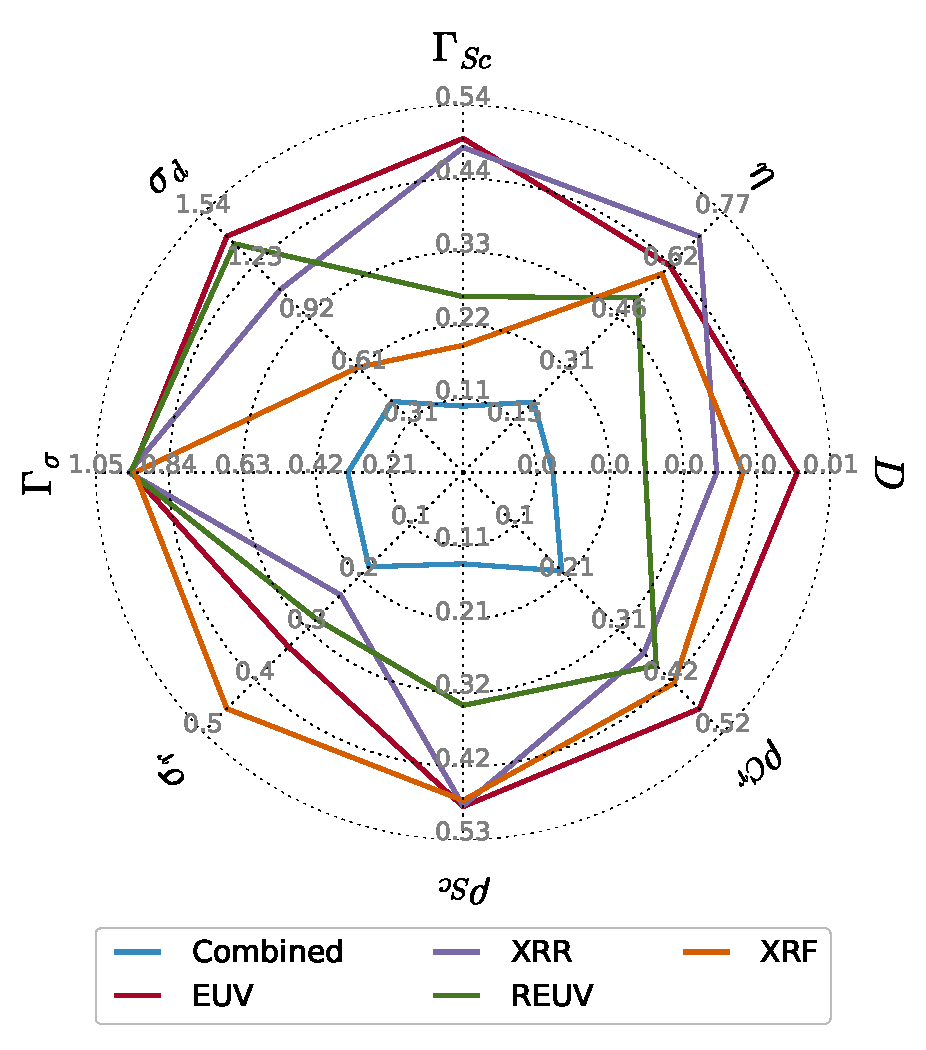
\includegraphics[width=0.6\textwidth]{images/spiderplot_confidence_intervals_empty}
  \caption{Visualization of the total confidence intervals for each of the parameters with respect to each of the individual experiments as well as the combined analysis.}
  \label{fig:confidence_intervals}
\end{figure}
It is worth noting that the confidence interval for the combined analysis is significantly smaller compared to the individual experiments. This is especially true for the parameter $\Gamma_\sigma$ describing the asymmetry of the interdiffusion layers. Within each of the individual experiments this parameter remains undefined, while the combined analysis delivers significant result of clearly asymmetric interdiffusion layer thicknesses.


\section{Results and Discussion}

The best fit result based on the two-step optimization procedure of the combined data set of all experiments are shown in Fig.~\ref{fig:combined_fit_result} together with the experimental data. The theoretical calculations based on the above model and the experimental data show a good agreement. Nevertheless, differences can be observed. The reason lies in the fact that each experiment was conducted in different experimental setups. Additionally, the beam divergence could not be considered in the analysis of the XRF experiment leading to less pronounced curve shapes in the experimental data than in the theoretical calculations. These deviations affect the confidence intervals given in Table~\ref{tbl:results} and are therefore taken into account. They lead to an increase the uncertainty of the end result.
\todo{Maybe it is possible to give uncertainty values for the best case? perfect homogeneous sample?}
\onecolumn
\begin{figure}
  \centering
  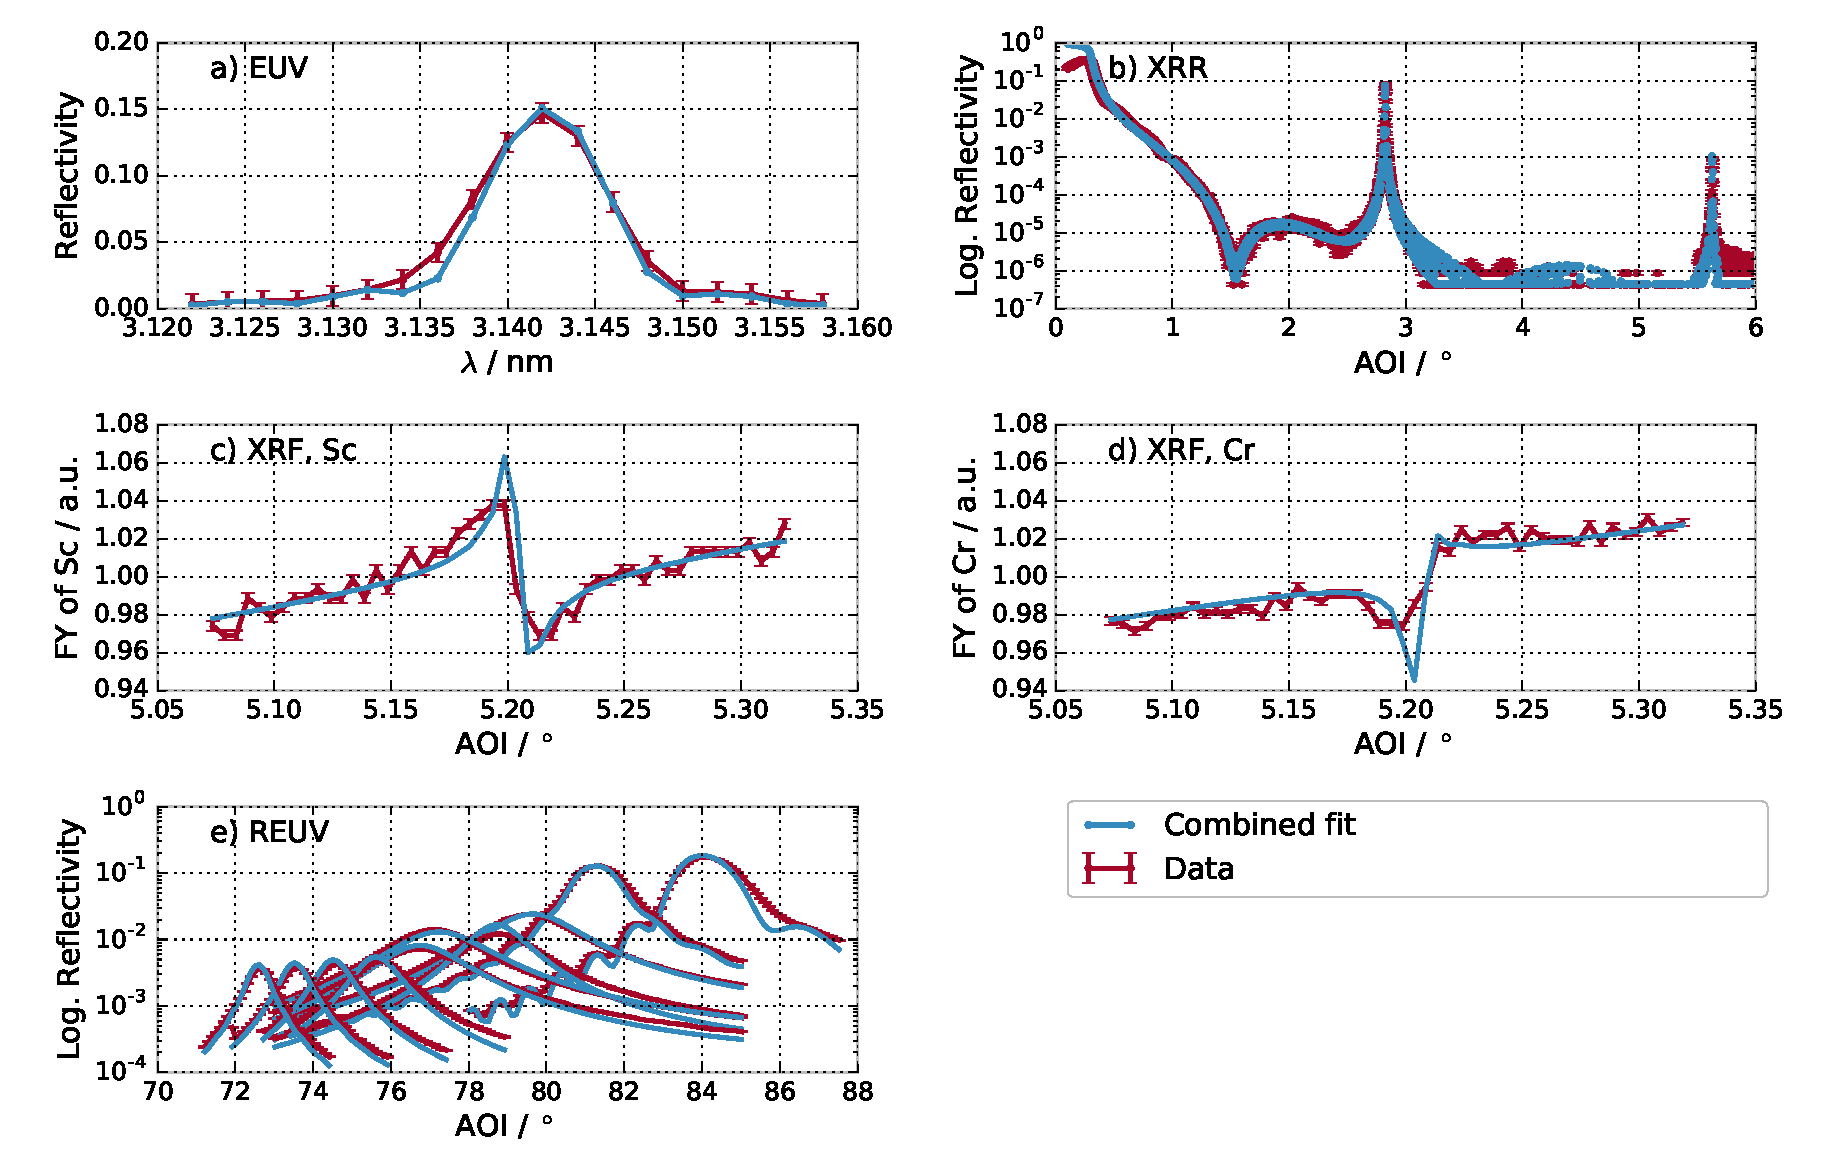
\includegraphics[width=0.9\textwidth]{images/combined_fit_result}
  \caption{Measured and calculated reflectivity and intensity curves for the optimized parameters with the combined analysis of all experiments as listed in Table~\ref{tbl:parametrization}.}
  \label{fig:combined_fit_result}
\end{figure}
\twocolumn
The electron density profile, i.e.~the depth dependence of the index of refraction, can now be constructed explicitly by applying the optimal parameters to the model. The result is shown in Fig.~\ref{fig:electron_density_profile} together with the initial binary model for comparison.
\begin{figure}
  \centering
  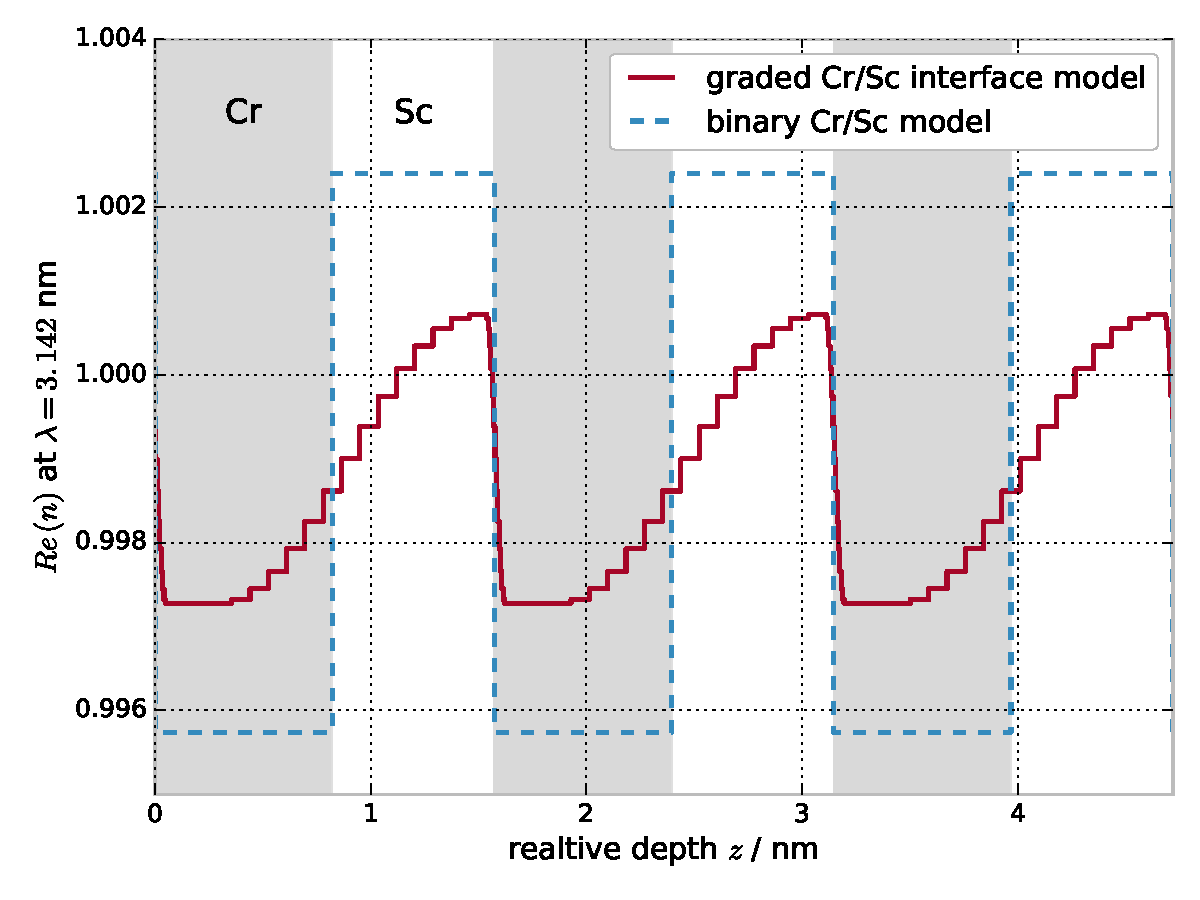
\includegraphics[width=\textwidth]{images/real_model}
  \caption{Real part of the index of refraction $n$  based on the results of the optimized parameters listed in Table~\ref{tbl:results} for the combined analysis for a selected wavelength. The gradual interface model is shown in direct comparison to the binary model optimized for the EUV reflectivity curve over three full periods. The resulting strong asymmetry in the width of the interface regions is clearly visible (see text). The gray and white shaded areas indicate the Cr and Sc layers, respectively, for the binary model.}
  \label{fig:electron_density_profile}
\end{figure}
An asymmetric distribution of the interdiffusion layers can be observed. This result is only possible due to the combination of all analytic experiments conducted here, as can be seen from the confidence intervals in Fig.~\ref{fig:confidence_intervals} as well as the values in Table~\ref{tbl:results}. A possible physical reason for this effect is the deposition process through magnetron sputtering. The elements Cr and Sc have different mass and thus different momentum when deposited onto each other. A similar effect is known from the deposition of Mo/Si multilayer systems, where the heavier Mo shows higher penetration into the Si layer than vice versa \cite{mosi_asymmetry}. In case of Cr/Sc multilayers, the Cr is heavier and thus has higher momentum leading to a broader interdiffusion layer.
The validation using the MCMC procedure also yield possible correlations between single parameters of the model. In case of the data, methods and model presented here even the combined analysis leaves a correlation between the intermixing parameter $\eta$ and the roughness $\sigma_r$. This means that none of the methods, not even the combined analysis contains sufficient information to deduct a unambiguous result for the roughness or intermixing. Intermixing alone merely reduces optical contrast, while interface roughness causes diffuse scattering. A natural tool for distinguishing between the two is thus provided through the measurement of the diffuse scattering. The distribution of the off-specular scattering with respect to the angle and wavelength provide additional information on the vertical and lateral correlation of spacial roughness frequencies. The latter is described by the power spectral density. We conducted a diffuse scattering experiment as described in Sec.~\ref{sec:experimental}. The analysis was done based on the DWBA formalism outlined in Sec.~\ref{sec:matrix_formalism}. The left-hand side of Fig.~\ref{fig:diffuse_meas} shows the measured reciprocal space map in direct comparison to the best-model found within the DWBA approach. The formation of a narrow Bragg sheet \cite{Haase:14,PhysRevLett.73.2228} confirms the high degree of roughness correlation and thereby justifies the approximations made in Sec.~\ref{sec:matrix_formalism} for identical roughness properties at each interface. To deduct the effective power spectral density shown on the right hand side of Fig.~\ref{fig:diffuse_meas} we have taken a cut along the Bragg sheet as indicated by the dashed white lines in the reciprocal space maps and divided it by the multilayer enhancement factor in Eq.~\ref{eqn:dwba} leaving the contribution of the effective PSD $C(q_x)$ to the diffuse scattering.
\onecolumn
\begin{figure}
  \centering
  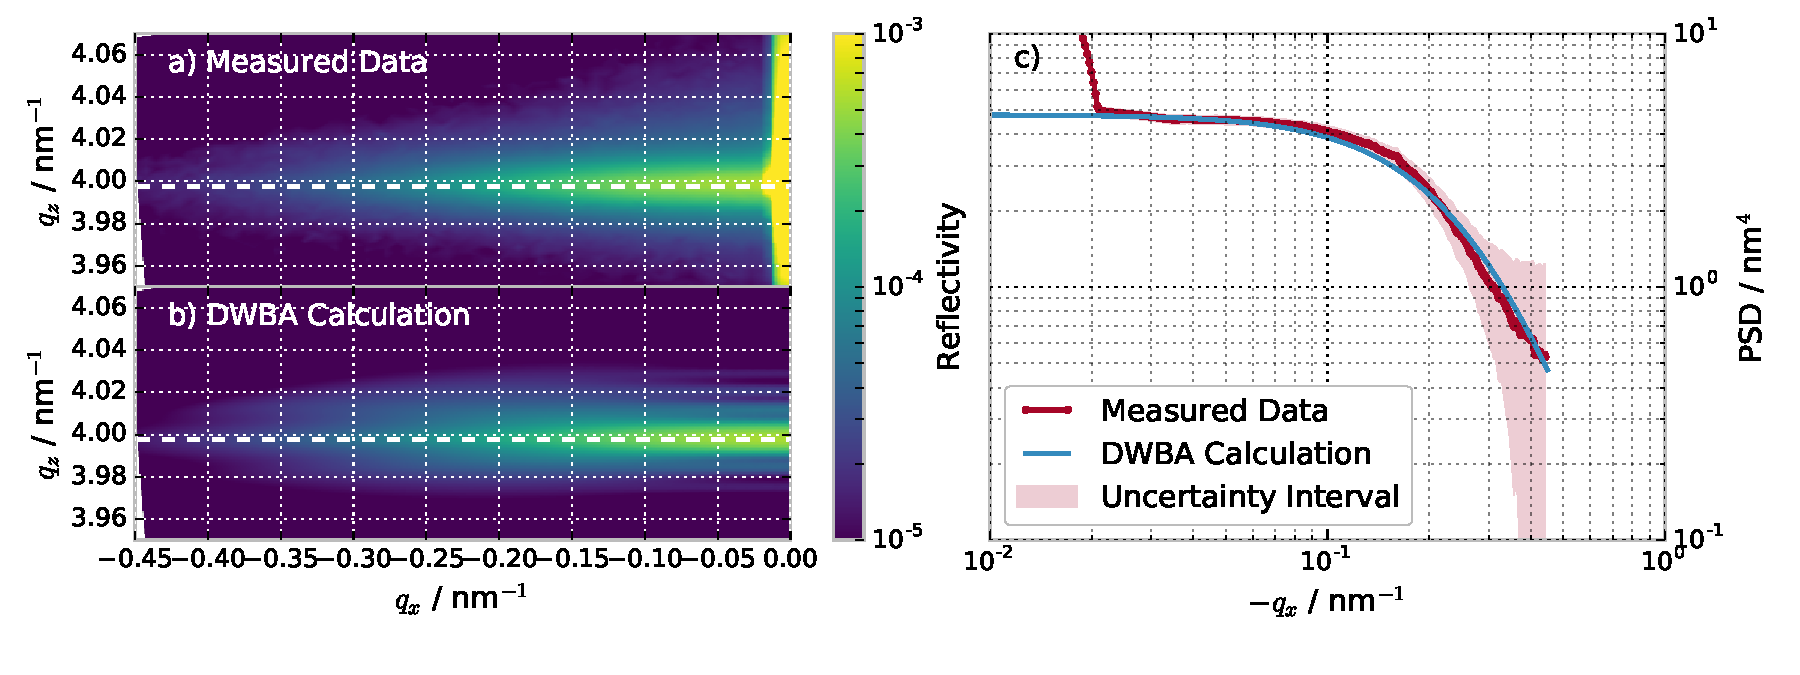
\includegraphics[width=\textwidth]{images/diffuse_incl_psd}
  \caption{a) Diffuse scattering measurement in $q$-space representation and log scale. b) DWBA Calculation of the optimal PSD model based on the electron density profile with the multilayer parameters for the combined analysis listed in Table~\ref{tbl:results}. c) Comparison of the extracted effective PSDs from the diffuse scattering measurement shown in (a) and the calculation of (b) at the horizontal cut positions indicated by the white dashed lines. The uncertainty interval for the extracted measured data is also indicated.}
  \label{fig:diffuse_meas}
\end{figure}
\twocolumn
The best-model results for the vertical replication factor and the power spectral density are given in Table.~\ref{tbl:psd_results}.

\begin{table}
\centering
\caption{Intervals of the parameters entering the PSO procedure}
\label{tbl:psd_results}
\begin{tabular}{@{}ll@{}}
\toprule
Parameter & Best model values\\ \midrule
$\sigma_r$ / nm & $0.187$ \\
$\xi_\parallel$ / nm& $3.3$ \\
$\xi_\perp$  / nm& $7.0$ \\
$H$ & $1.0$ \\
$\beta$ & $0.0$ \\
 \bottomrule
\end{tabular}
\end{table}

\section{Conclusions}

In conclusion we have demonstrated a robust method to characterize ultra-thin multilayer systems with sub-nanometer layer thicknesses unambiguously. Layer thicknesses in the sub-nanometer regime are necessary for near-normal incidence reflective mirrors in the water window spectral range. However, they come with the cost of increasing susceptibility to disturbances of the interfaces at the layer boundaries. This limits the achievable reflectivity to values well below the theoretical threshold posing a demand for ideally non-destructive characterization methods. The main mechanisms diminishing reflectivity are interdiffusion and roughness. With these effects ranging in the order of the layer thickness models based on binary layer stacks become inadequate to describe the physical situation. In order to find a proper representation of the multilayer sample more sophisticated models with explicit description of the gradual interdiffusion layers become necessary. This inevitably increases the numbers of parameters of the describing model to be determined in analytical experiments. We performed a rigorous analysis of several analytic methods to determine the model parameters representing the sample. Finding a unambiguous solution is challenging and can only be achieved with a combined analysis of several non-destructive techniques. The optimal set of parameters was determined by applying a particle swarm optimizer in conjunction with a Markov-chain Monte Carlo method to verify the uniqueness of the solution and derive confidence intervals for all parameters in all experiments. The set of analytical methods we employed were EUV and X-ray reflectivity, resonant EUV reflectivity across the Sc L-edge as well as X-ray standing wave fluorescence at the Sc and Cr K-lines across the first Bragg peak. The analysis of each method shows the different sensitivities for specific parameters of the model. The EUV reflectivity shows sensitivity for the optical contrast, i.e. the intermixing $\eta$ and the roughness $\sigma_r$. With the resonant EUV reflectivity this is further improved and additional sensitivity is added with respect to the ratio of Sc and Cr as well as the total period thickness $D$. The XRR measurement on the other hand yields small confidence intervals for the roughness $\sigma_r$ and also the periodicity $D$. Finally, XRF delivers a method to resolve the multilayer structure spacially and thus the interdiffusion layer thickness $\sigma_d$ and the Sc to Cr ratio. With the combination of all these methods a robust result could be derived with small confidence intervals. Most notably, only the combined analysis can detect the asymmetry of the interdiffusion layers $\Gamma_\sigma$.

Within the small confidence intervals the MCMC methods yields only a single remaining correlation of the intermixing parameter and the roughness factor, which could not be resolved with the experiments in specular geometry. In addition to the combined analysis we therefore added a measurement of the off-specular diffuse scattering to distinguish between the roughness and the interdiffusion. The results of this analysis reveal a high degree of roughness correlation throughout the multilayer with r.m.s.~values comparable with the best fit obtained in the combined analysis and AFM measurements on the top surface layer (not shown here).

     %-------------------------------------------------------------------------
     % The back matter of the paper - acknowledgements and references
     %-------------------------------------------------------------------------

     % Acknowledgements come after the appendices

%\ack{Acknowledgements}

     % References are at the end of the document, between \begin{references}
     % and \end{references} tags. Each reference is in a \reference entry.


%% Note added by Overleaf: If using bibtex, remove the "references" environment above, and uncomment the following lines.
\bibliographystyle{iucr}
\bibliography{references_nourl}

\end{document}                    % DO NOT DELETE THIS LINE
%%%%%%%%%%%%%%%%%%%%%%%%%%%%%%%%%%%%%%%%%%%%%%%%%%%%%%%%%%%%%%%%%%%%%%%%%%%%%%
